% !TeX root = ./PhDThesis.tex

\chapter{Experimental realization of a 200-ion multi-qubit quantum memory}

Storage lifetime and capacity are two important factors to characterize the performance of a quantum memory, which finds wide applications in quantum computers and quantum networks. The trapped ion system has reported the longest single-qubit storage lifetime above one hour, as well as the multi-qubit capacity up to tens of ions in shallow-depth quantum circuits. However, combining the two features still remains an experimental challenge due to the stronger noise in the multi-qubit environment. Here we report the stable trapping of above 200 ions in a zigzag structure, and demonstrate the combination of the multi-qubit capacity and long storage lifetime by measuring the coherence time of several arbitrarily chosen ions to be on the order of hundreds of milliseconds. We compare the performance of the quantum memory with and without the sympathetic cooling laser, thus unambiguously show the necessity of sympathetic cooling for the long-time storage of multiple ionic qubits.



\section{Quasi-1D ion crystal}

\begin{figure}
    \centering
    \includegraphics[width=0.5\linewidth]{fig_6_1_a.pdf}
    \caption{Schematic experimental setup.}
    \label{fig:6_1_a}
\end{figure}

To get a stable quasi-1D ion crystal, we use a blade trap in a closed-cycle cryostat at a temperature of $6\,$K. As shown in Fig.~\ref{fig:6_1_a}, a 1D or quasi-1D ion crystal is confined in a blade trap under cryogenic temperature. A broad elliptic beam with tunable frequency and intensity can be used for global Doppler cooling, optical pumping and qubit state detection, and a narrow sympathetic cooling beam propagating in the opposite direction can address about 5 central ions. A microwave horn antenna generates microwave signals to manipulate the states of the qubits. We apply a global Doppler cooling beam with nonzero angles to all the three principle axes. This global beam has $20\,\upmu$W power and $\Delta=-2\pi\times 12\,$MHz detuning, and is shaped into an ellipse with waist sizes of $15\,\upmu$m$\times 500\,\upmu$m by a cylindrical lens. Opposite to this beam is a narrow $1\,\upmu$W sympathetic cooling beam with the same detuning, which is focused to a beam waist of $10\,\upmu$m to address about 5 ions in the center of the crystal. By setting the transverse trap frequencies $\omega_x\approx 1.6\,$MHz, $\omega_y\approx 1.5\,$MHz, and by engineering the axial trapping potential via the segmented electrodes (for the long ion crystal, the axial potential cannot be well approximated by a harmonic trap), we obtain a quasi-1D ion crystal of 218 $^{171}\mathrm{Yb}^+$ ions in a zigzag shape, which can be stably trapped for hours under the global cooling beam.

\begin{figure}
    \centering
    \includegraphics[width=1.0\linewidth]{fig_6_1_b.pdf}
    \caption{The image of 218 ions in a zigzag structure.}
    \label{fig:6_1_b}
\end{figure}

An image of the 218 ions is shown in Fig.~\ref{fig:6_1_b}. The length of this quasi-1D crystal is about $800\,\upmu$m and is wider than the FOV of the EMCCD camera of about $300\,\upmu$m, so the image is stitched from three images taken sequentially with overlap in between. The blue arrows indicate the locations of five dark ions. The ions labelled as 1, 2 and 3 are used to demonstrate quantum storage in the following experiments. For an illustration of the whole ion crystal, we take photos sequentially for different parts of the ion crystal by shifting the position of the camera, and perform image stitching to combine them together. In the following when characterizing the storage capacity and the lifetime of the quantum memory, we apply sympathetic cooling laser to the middle ions and store and read out qubit states on the edge, so that the shifting of the camera position is not needed.



\section{Measure the storage time}

\begin{figure}
    \centering
    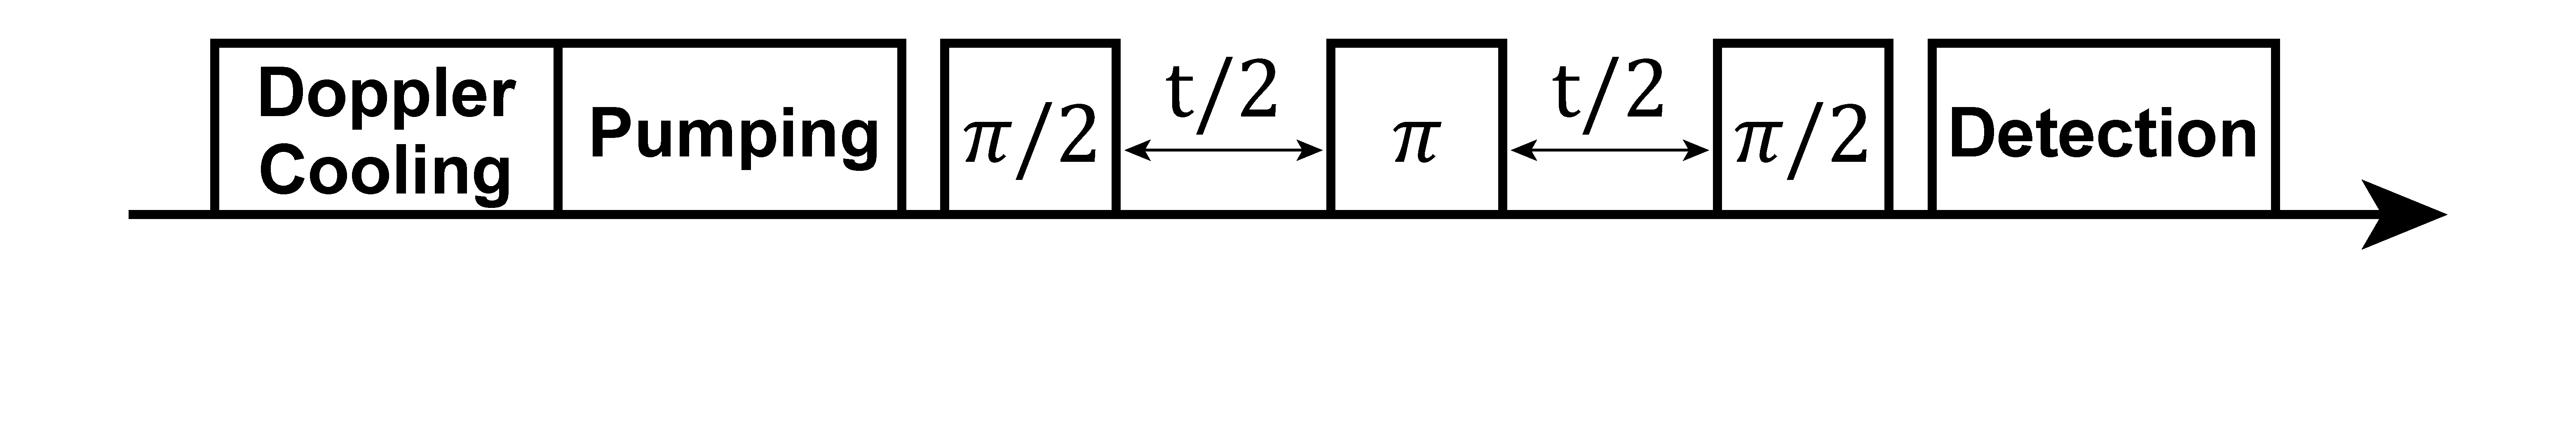
\includegraphics[width=0.5\linewidth]{fig_6_1_c.pdf}
    \caption{Experimental sequence.}
    \label{fig:6_1_c}
\end{figure}

We apply a global microwave to manipulate the qubit states through the spin-echo sequence shown in Fig.~\ref{fig:6_1_c}. We initialize the storage qubit in $|0\rangle \equiv |^{2}\mathrm{S}_{1/2},F=0,m_F=0\rangle$ of the $^{171}\mathrm{Yb}^+$ ion (a dark state under $370\,$nm detection laser) through optical pumping, and apply a $\pi/2$ pulse to prepare it in $(|0\rangle+e^{i\phi}|1\rangle)/\sqrt{2}$ where $\phi$ is the initial phase of the microwave signal. After the long-time storage with a spin echo (microwave $\pi$ pulse) in the middle, we apply another microwave pulse to reverse the preparation step and finally measure the storage fidelity of the qubit state. Due to the nonuniformity of the microwave, we use SK1 composite pulses for the $\pi/2$ and $\pi$ pulses to suppress the pulse area error. Ideally we will end in the state $|1\rangle \equiv |^{2}\mathrm{S}_{1/2},F=1,m_F=0\rangle$ (a bright state under the detection laser), and the decay in the population versus time can give us the storage lifetime of the quantum memory.

\begin{figure}
    \centering
    \subcaptionbox{Rabi oscillation of the ion on the left side of the ion chain.\label{fig:6_2_a}}
    {\includegraphics[width=0.4\linewidth]{fig_6_2_a.pdf}}
    \subcaptionbox{Rabi oscillation of the ion on the right side of the ion chain.\label{fig:6_2_b}}
    {\includegraphics[width=0.4\linewidth]{fig_6_2_b.pdf}}
    \subcaptionbox{Compare theoretical and experimental performance for the single pulse.\label{fig:6_2_c}}
    {\includegraphics[width=0.5\linewidth]{fig_6_2_c.pdf}}
    \caption{Usage of the SK1 composite pulse.}
    \label{fig:6_2}
\end{figure}

Due to the nonuniformity of the microwave signal, its Rabi frequency varies slightly for different ions, so we use the SK1 composite pulse to suppress this pulse-area error to higher order. As shown in Fig.~\ref{fig:6_2}, there is about $30\%$-$40\%$ change in the Rabi frequency over 80 ion spacings, or about $0.5\%$ change between adjacent ions, and the SK1 pulse can tolerate up to $\pm20\%$ error in the Rabi frequency while still maintaining a fidelity above $99\%$. Here we use the Rabi oscillation of different sites in a chain of about 100 ions to characterize the nonuniformity of the microwave signal. For two ions separated by 80 ion spacings, the Rabi frequencies of Fig~\ref{fig:6_1_a} $2\pi\times 10.3\,$kHz and Fig~\ref{fig:6_1_b} $2\pi\times 7.4\,$kHz are fitted. Fig~\ref{fig:6_1_c} shows theoretical (solid curves) and experimental (dots) performance for the single pulse (blue) and the composite pulse (red) on a target ion. Theoretically, the SK1 composite pulse can tolerate up to $\pm 20\%$ pulse-area error while still maintaining a fidelity above $99\%$. Similar tendency is observed in the experiment and the overall reduction in the fidelity can be explained by the state-preparation-and-measurement (SPAM) error. Therefore, we can simultaneously initialize all the ions in the FOV of the CCD camera in the same state and operate them with the same gate, which allows efficient characterization of their storage lifetime without the need to repeat the experimental sequence for each ion. Note that here our purpose is to demonstrate the storage capacity and lifetime of individual ions in the crystal, so global operations plus individual detection suffice. In the future with an upgrade in the addressing system using focused Raman laser beams, the simultaneous storage of multiple qubits into nearby ions can also be achieved.

\begin{figure}
    \centering
    \subcaptionbox{Storage time for the 1st ions.\label{fig:6_3_a}}
    {\includegraphics[width=0.4\linewidth]{fig_6_3_a.pdf}}
    \subcaptionbox{Storage time for the 16th ions.\label{fig:6_3_b}}
    {\includegraphics[width=0.4\linewidth]{fig_6_3_b.pdf}}
    \subcaptionbox{Storage time for the 31st ions.\label{fig:6_3_c}}
    {\includegraphics[width=0.4\linewidth]{fig_6_3_c.pdf}}
    \subcaptionbox{The decay of the bright state population vs. storage time without the spin echo.\label{fig:6_3_d}}
    {\includegraphics[width=0.4\linewidth]{fig_6_3_d.pdf}}
    \caption{The measured storage fidelity vs. storage time.}
    \label{fig:6_3}
\end{figure}

We measure the storage lifetime of three typical ions [labeled as 1-3 in Fig.~\ref{fig:6_1_b}] away from the center of the ion crystal in Fig.~\ref{fig:6_3}(a)-(c). By executing the pulse sequence in Fig.~\ref{fig:6_1_c}, we get the average storage fidelity over the $|\pm\rangle=(|0\rangle\pm|1\rangle)/\sqrt{2}$ and $|L(R)\rangle=(|0\rangle\pm i|1\rangle)/\sqrt{2}$ bases, and fit the decoherence time $T_2=(323\pm 93)\,$ms, $(453\pm218)\,$ms and $(419\pm104)\,$ms, respectively, for the three ions. The coherence time $T_2$ is fitted by the exponential function $F=A+Be^{-t/T_2}$. Each data point is repeated for 200 times with the error bar indicating one standard deviation. At large $t$, some data points deviate considerably from the exponential fitting function. This can be explained by the slow drift in the trap and laser parameters on the timescale of minutes to hours, and should not affect the extracted coherence time of hundreds of milliseconds. Nevertheless, a coherence time on the order of hundreds of milliseconds can be concluded. On the other hand, the $|0(1)\rangle$ basis is not subjected to the dephasing error and hence typically have longer coherence time. For example, in Fig.~\ref{fig:6_3_d} we see that, without the spin echo in the middle which does not affect the decoherence in the $|0(1)\rangle$ basis, the population decay from the bright state ($|1\rangle$) to the dark state ($|0\rangle$) for a typical ion has a timescale far above $1\,$s. Therefore we can bound the average storage lifetime over all possible qubit states by $T_2$ for individual ions.



\section{Effect of the sympathetic cooling}

\begin{figure}
    \centering
    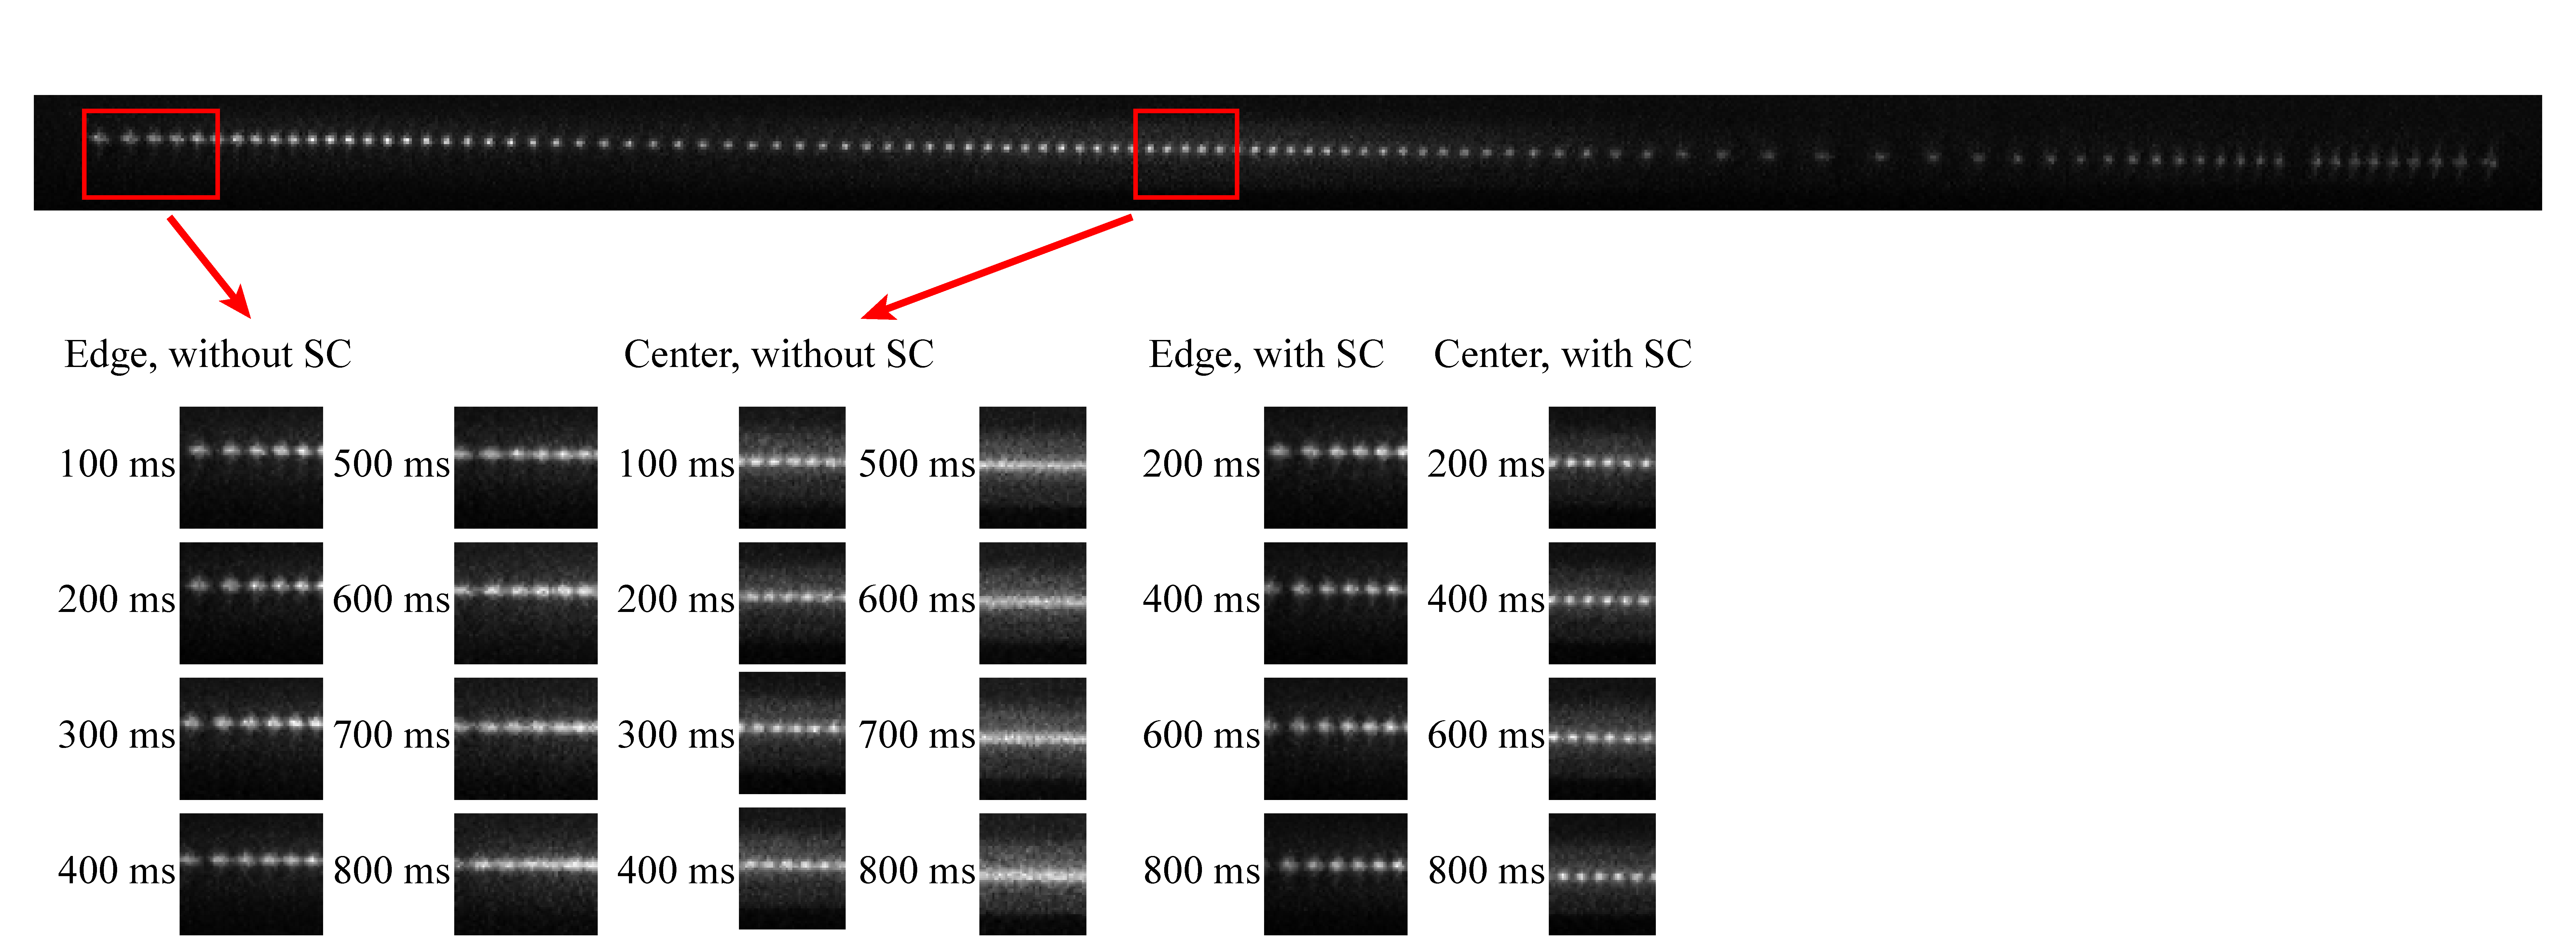
\includegraphics[width=1.0\linewidth]{fig_6_4_abc.pdf}    \caption{Compare the heating effect with or without sympathetic cooling.}
    \label{fig:6_4_abc}
\end{figure}

The sympathetic cooling laser beam turns out to be critical for the functioning of this quantum memory: without the cooling beam, the ion crystal can quickly be heated up within hundreds of milliseconds that can cause difficulty in reading out the qubit state or even the meltdown of the whole ion crystal. Actually, for the quasi-1D 218-ion crystal, the heating dynamics is too fast to be examined from the images. Therefore we first demonstrate the idea using a shorter chain of about 100 ions whose heating dynamics is slower.

The image of a 1D 103-ion chain under the same parameters as those for the crystal is shown in Fig.~\ref{fig:6_4_abc}. To compare the heating effect with or without sympathetic cooling, we start from the same equilibrium state under global Doppler cooling, and then turn off the global cooling beam and evolve the system with the sympathetic cooling (SC) beam off or on. Each image is averaged over 200 repetitions.

The two columns on the left show the images of the edge ions and the central ions [indicated by the red boxes in (a)] with the sympathetic cooling beam turned off. As the heating dynamics proceeds, the spots of individual ions dim and expand, making it difficult to detect individual qubit states. The two columns on the right show the images of the same edge ions and the same central ions with the sympathetic cooling beam turned on. There is no visible change in these images after $800\,$ms evolution. We can conclude that without the sympathetic cooling, the spots of individual ions quick blur and mix up with each other. This process is fastest for the middle ions with small inter-ion distances, but even for ions on the edges it will finally become difficult to distinguish individual ions. On the other hand, with the sympathetic cooling beam turned on, the ions remain distinguishable and there is no visible change over $800\,$ms evolution time.

\begin{figure}
    \centering
    \includegraphics[width=0.5\linewidth]{fig_6_4_d.pdf}    \caption{The decay of photon counts.}
    \label{fig:6_4_d}
\end{figure}

With this basic understanding about how the heating effects damage the qubit state detection, now we apply it to the 218-ion crystal. In Fig.~\ref{fig:6_4_d} we pick up an ion (labeled as ion 1 above) and measure the photon counts in a $5\,$pixels$\times5\,$pixels box around it. With the sympathetic cooling beam turned off, the photon count quickly decays within $100\,$ms, and we estimate a decay time of $\tau=(256\pm14)\,$ms from the simplest fitting model of $e^{-t/\tau}$. This decay comes from two effects: as the ion heats up, it is more likely to move outside the selected region, and it scatters less photons due to the larger Doppler shifts. In the experiment, we use a threshold method to distinguish the bright ($|1\rangle$) and the dark ($|0\rangle$) state. Therefore the drop in the photon count of the bright state will significantly reduce the detection fidelity even before the timescale $\tau$, and is shorter than the coherence time $T_2$ measured before under sympathetic cooling.

Although we show that sympathetic cooling is critical for the long-time storage of the qubit states in the multi-ion crystal, it is also well-known that the scattered photons from the cooling ions can lead to crosstalk on the storage ions and thus limit the storage lifetime. This is because of the same transition frequency between the cooling ions and the storage ions. Previously, this is solved by using different ion species to encode the two qubit types. In the future, when combined with the dual-type qubit scheme which encodes the data qubits and the ancilla qubits into different clock states of the same ion species, the crosstalk can be suppressed to allow smaller distance between the two qubit types and an enhanced storage lifetime, without the need to manipulate multiple ion species.

To sum up, we have demonstrated the multi-ion storage capacity with sub-second lifetime in a quasi-1D crystal of above 200 ions. This capability to coherently store a large number of qubits for long time is crucial for the quantum computing tasks in the future with deep circuit depth. It is also necessary for ion-photon quantum networks since the entanglement generation between different ion trap modules through photon links is typically much slower than the local gate operations inside individual modules.
